\documentclass{article}
\usepackage{graphicx} % Required for inserting images
\usepackage{biblatex}
\usepackage{hyperref}
\usepackage{amssymb}
\usepackage{amsmath}
\usepackage{float}
\hypersetup{pdfborder=0 0 0}
\usepackage[a4paper, margin=1in]{geometry}
\usepackage{gensymb}
\usepackage{pdfpages}

\title{\Large \textbf{ECE 66100 Homework \#1\\[0.1in] by\\ [0.1in] Adrien Dubois (dubois6@purdue.edu)}}

\begin{document}

\maketitle
\section*{Problem 1:}
The following lemma will be used for the solution to this problem.

% Beginning of lemma
\subsection*{Lemma 1:} Let the vector $\boldsymbol{\Vec{v}}$ be the homogeneous representation of the physical point $\boldsymbol{\Vec{x}}$. It is known that the 3D vector \(\boldsymbol{\Vec{v}} = \begin{bmatrix}
    x \\ y \\ 1
\end{bmatrix} \in \mathbb{R}^3\) is the homogeneous coordinate representation of a physical 2D point in \((x, y) \in \mathbb{R}^2\). 

\subsection*{Lemma 2:} Using lemma 1, we note that every \(k \times \boldsymbol{\Vec{v}} = k \times \begin{bmatrix}
    x \\ y \\ 1
\end{bmatrix}, k\in\mathbb{R}, k \neq 0\) is the same physical point \((x,y)\in \mathbb{R}^2\). We can therefore denote a new general representation for the homogeneous coordinate form a physical point in $\mathbb{R}^2$: 
\[
\boldsymbol{\Vec{v}} = 
\begin{bmatrix}
    u \\ v \\ w
\end{bmatrix} \text{ where } x = \frac{u}{w} \text{ and } y = \frac{v}{w}\]

% End of lemma
\subsection*{Solution:}
We can represent the point at origin in the physical space $\mathbb{R}^2$ by: 
\[\boldsymbol{\Vec{x_0}} = 
    \begin{bmatrix}
        x_1 \\ x_2
    \end{bmatrix}
= \begin{bmatrix}
    0 \\ 0
\end{bmatrix}\]

Therefore, using lemma 1 we can convert \(\boldsymbol{\Vec{x_0}}\) into its homogeneous coordinate representation: \[\boldsymbol{\Vec{x_0}} = \begin{bmatrix}
    x \\ y \\ 1
\end{bmatrix} = \begin{bmatrix}
    0 \\ 0 \\ 1
\end{bmatrix}\]

Lastly, by corollary from lemma 2 and the previous result, we can find the generalized version of this point using lemma 2. These are all the points in the homogeneous coordinate system in $\mathbb{R}^3$ that represent the origin the physical space:
\[\boldsymbol{\Vec{x_0}} = \begin{bmatrix}
    0 \\ 0 \\ w
\end{bmatrix} \text{ where } w \in \mathbb{R} \text{ and } w \neq 0\]

\newpage
\section*{Problem 2:}
The following definitions will be utilized in the solution to problem 2.

\subsection*{Definition 1: Representation of a line in homogeneous coordinates} 

In the physical space $\mathbb{R}^2$, we can represent an arbitrary line $\boldsymbol{line_1}$ as follows: 
\[\boldsymbol{line_1}: ax + by + c = 0 \text{ for some arbitrary values: } a,b,c \in \mathbb{R}\]

This line will therefore have a slope of $\frac{-a}{b}$ and will intercept the y-axis at point: $(0, \frac{-c}{b})$.

Next, considering the vector representation of the line's parameters: 
\[\boldsymbol{\Vec{l_1}} = \begin{bmatrix}
    a \\ b \\ c
\end{bmatrix}\]

we can represent the algebraic equation of the line $\boldsymbol{l_1}$ in the homogeneous coordinate system as follows: 
\[\boldsymbol{line_1}: \boldsymbol{\Vec{l_1}}^T x = 0 \text{ or } \boldsymbol{\Vec{l_1}} x^T = 0 \text{ where } x = \begin{bmatrix}
    x \\ y \\ 1
\end{bmatrix}\]

\subsection*{Lemma 3: The intersection of 2 lines in HC}
Given two lines represented in homogeneous coordinates: \(l_1 = \begin{bmatrix}
    a_1 \\ b_1 \\ c_1
\end{bmatrix}\) and \(l_2 = \begin{bmatrix}
    a_2 \\ b_2 \\ c_2
\end{bmatrix}\), the point of intersection (x) between the two lines is their vector cross product: \(x = l_1 \times l_2\).

\subsection*{Solution:}
We can define a point at infinity by the point of intersection of two different, parallel lines $\boldsymbol{line_1} \text{ and } \boldsymbol{line_2}$ parameterized by the following vectors:
\[
\boldsymbol{\Vec{l_1}} = \begin{bmatrix}
    a \\ b \\ c_1
\end{bmatrix}
\text{ and } \boldsymbol{\Vec{l_2}} = \begin{bmatrix}
    a \\ b \\ c_2
\end{bmatrix}\]

We can confirm that these two lines are different and parallel since they have equal slopes: $m = \frac{-a}{b}$ and different y-intercepts: $(0, \frac{-c_1}{b} \text{ and } \frac{-c_2}{b})$

Using lemma 3, we can now calculate the point of intersection (x) between $\boldsymbol{line_1} \text{ and } \boldsymbol{line_2}$:
\[
x = \boldsymbol{\Vec{l_1}} \times \boldsymbol{\Vec{l_2}} = \begin{bmatrix}
    b \\ -a \\ 0
\end{bmatrix}
\]

Now consider two new, different and parallel lines $\boldsymbol{line_3} \text{ and } \boldsymbol{line_4}$ with the following representations in H.C.:
\[
\boldsymbol{\Vec{l_3}} = \begin{bmatrix}
    \alpha \\ \beta \\ c_3
\end{bmatrix}
\text{ and } \boldsymbol{\Vec{l_4}} = \begin{bmatrix}
    \alpha \\ \beta \\ c_4
\end{bmatrix} \text{ where } \alpha x + \beta y \neq k (ax + by), k\in\mathbb{R}, k\neq 0\]

Following the previous reasoning, these lines will also meet at infinity. This point of intersection will be: 
\[
    x'= \boldsymbol{\Vec{l_3}} \times \boldsymbol{\Vec{l_4}} = \begin{bmatrix}
    \beta \\ -\alpha \\ 0
\end{bmatrix} \neq \begin{bmatrix}
    b \\ -a \\ 0
\end{bmatrix}
\]

Hence, it has been showed that not all points at infinity in the physical plane $\mathbb{R}^2$ are the same. Instead, these points all lie on the same line at infinity in the homogeneous coordinate system, and the direction at which they approach infinity is controlled by the slope of the line parameterized by their coordinate in HC.

\newpage
\section*{Problem 3:}
\subsection*{Definition 2: General Conic in HC}
It is known that the representation of a conic in the physical space $\mathbb{R}^2$ is: 
\[\text{\textbf{Equation 1: }} ax^2 + bxy + cy^2 + dx + ey + f = 0\]

Following the procedure in \textbf{Definition 1}, we can express the previous equation in homogeneous coordinates by representing the point $(x,y)$ as \(\begin{bmatrix}
    x_1 \\ x_2 \\ x_2
\end{bmatrix}\) where \(x = \frac{x_1}{x_3}\) and \(y = \frac{x_2}{x_3}\). Using this representation, we can rewrite \textbf{Equation 1} as follows:
\[\text{\textbf{Equation 2: }} ax_1^2 + bx_1x_2 + cx_2^2 + dx_1x_3 + ex_2x_3 + fx_3^2 = 0\]
Which is the same as the following vector-matrix product:
\[\begin{bmatrix}
    x_1 & x_2 & x_3
\end{bmatrix} \begin{bmatrix}
    a & \frac{b}{2} & \frac{d}{2} \\
    \frac{b}{2} & c & \frac{e}{2} \\
    \frac{d}{2} & \frac{2}{2} & f
\end{bmatrix} \begin{bmatrix}
    x_1 \\ x_2 \\ x_3
\end{bmatrix} = 0
\]

Therefore, every conic must satisfy the equation: \(\boldsymbol{\Vec{x}}^T \boldsymbol{C} \boldsymbol{\Vec{x}} = 0\) where C is the non-singular, symmetrical matrix shown above.

\subsection*{Definition 3: Degenerate Conic in HC}
A degenerate conic is a subset of the general conic that occurs when the slice a double cone with a plane that passes through its axis. This will result in two lines which we will denote: $l$ and $m$

Since every point on the degenerate conic C is on $l$ or $lm$, the definition of C in HC is given by:
\[\boldsymbol{C} = \boldsymbol{\Vec{l}} \boldsymbol{\Vec{m}}^T + \boldsymbol{\Vec{m}} \boldsymbol{\Vec{l}}^T\]

\subsection*{Lemma 4: Rank of the sum of two matrices}
It is known that if \textbf{A} and \textbf{B} are two $m \times n$ matrices, then rank(\textbf{A} + \textbf{B}) $\leq$ rank(\textbf{A}) + rank(\textbf{B}).


\subsection*{Solution}
From \textbf{Definition 2}, we know that the general definition of a conic C is: \(\boldsymbol{\Vec{x}}^T \boldsymbol{C} \boldsymbol{\Vec{x}} = 0\)

Using definition 3, we know that the degenerate conic C can be defined by \(\boldsymbol{C} = \boldsymbol{\Vec{l}} \boldsymbol{\Vec{m}}^T + \boldsymbol{\Vec{m}} \boldsymbol{\Vec{l}}^T\), where:
\[\boldsymbol{\Vec{l}} \boldsymbol{\Vec{m}}^T = \begin{bmatrix}
    l_1m_1 & l_1m_2 & l_1m_3 \\
    l_2m_1 & l_2m_2 & l_2m_3 \\
    l_3m_1 & l_3m_2 & l_3m_3 
\end{bmatrix} \text{ and } \boldsymbol{\Vec{m}} \boldsymbol{\Vec{l}}^T  = \begin{bmatrix}
    l_1m_1 & l_2m_1 & l_3m_1 \\
    l_1m_2 & l_2m_2 & l_3m_2 \\
    l_1m_3 & l_2m_3 & l_3m_3
\end{bmatrix}\]

It is trivial to see that the rows and columns of both \(\boldsymbol{\Vec{l}} \boldsymbol{\Vec{m}}^T\) and \(\boldsymbol{\Vec{m}} \boldsymbol{\Vec{l}}^T\) are linearly dependent. Therefore, by the definition of the rank function:
\[
Rank(\boldsymbol{\Vec{l}} \boldsymbol{\Vec{m}}^T) = 1 \text{ and } Rank(\boldsymbol{\Vec{m}} \boldsymbol{\Vec{l}}^T) = 1
\]. 

Lastly, by \textbf{Lemma 4}, we can determine that: 
\[Rank(C) = Rank(\boldsymbol{\Vec{l}} \boldsymbol{\Vec{m}}^T + \boldsymbol{\Vec{m}} \boldsymbol{\Vec{l}}^T) \leq Rank(\boldsymbol{\Vec{l}} \boldsymbol{\Vec{m}}^T) + Rank(\boldsymbol{\Vec{m}} \boldsymbol{\Vec{l}}^T) = 2
\]
\newpage
\section*{Problem 4:}
As stated in \textbf{Equation 2}, a conic can be defined as follows: \[ax_1^2 + bx_1x_2 + cx_2^2 + dx_1x_3 + ex_2x_3 + fx_3^2 = 0\]

We have also shown in \textbf{Definition 2} that the previous equation can be represented as such: 
\[\begin{bmatrix}
    x_1 & x_2 & x_3
\end{bmatrix} \begin{bmatrix}
    a & \frac{b}{2} & \frac{d}{2} \\
    \frac{b}{2} & c & \frac{e}{2} \\
    \frac{d}{2} & \frac{e}{2} & f
\end{bmatrix} \begin{bmatrix}
    x_1 \\ x_2 \\ x_3
\end{bmatrix} = 0
\]

From problem 4, we know that a conic will have: \(0 < Rank(C) \leq 3\), \(Rank(C) \in \mathbb{R}\). Therefore, we can determine that at least one of $a, c \text{ or } f$ will be non-zero. So, it can be factored out of the equation without affecting the conic since:
\[\boldsymbol{\Vec{x}}^T (k\boldsymbol{C}) \boldsymbol{\Vec{x}} = 0\]

\[k(\boldsymbol{\Vec{x}}^T \boldsymbol{C} \boldsymbol{\Vec{x}}) = 0\]
\[\boldsymbol{\Vec{x}}^T \boldsymbol{C} \boldsymbol{\Vec{x}} = \frac{0}{k} = 0 \text{ for } k\in\mathbb{R}, k\neq0\]

Applying this to the algebraic form of the conic C, we get:
\[a (x_1^2 + \frac{b}{a}x_1x_2 + \frac{c}{a}x_2^2 + \frac{d}{a}x_1x_3 + \frac{e}{a}x_2x_3 + \frac{f}{a}x_3^2) = 0\]
\[x_1^2 + \frac{b}{a}x_1x_2 + \frac{c}{a}x_2^2 + \frac{d}{a}x_1x_3 + \frac{e}{a}x_2x_3 + \frac{f}{a}x_3^2 = 0\]

This is an equation in 5 variables, so we would need 5 points to solve it. Therefore, at least 5 points are required to define a conic. 



\newpage
\section*{Problem 5:}
\subsection*{Step 1: Deriving the HC representation for line 1}
Since it is known that $\boldsymbol{l_1}$ passes through the points (0,0) and (3,4), we can find the definition of the line in homogeneous coordinates through the vector cross product of points 1 and 2:

\[\boldsymbol{l_1} = \begin{bmatrix}
    0 \\ 0 \\ 1
\end{bmatrix} \times \begin{bmatrix}
    3 \\ 4 \\ 1
\end{bmatrix} = \begin{bmatrix}
    -4 \\ 3 \\ 0
\end{bmatrix}\]

\subsection*{Step 2: Deriving the HC representation for line 2}
Following the same procedure, we can represent line 2 through the following forms:
\[\boldsymbol{l_2} = \begin{bmatrix}
    -1 \\ 4 \\ 1
\end{bmatrix} \times \begin{bmatrix}
    \frac{3}{2} \\ -1 \\ 1
\end{bmatrix} = \begin{bmatrix}
    5 \\ 5/2 \\ -5
\end{bmatrix}\]

\subsection*{Step 3: Find the intersection between both lines}
Lastly, the intersection point between $\boldsymbol{l_1}$ and $\boldsymbol{l_2}$, $\boldsymbol{\Vec{x}} = \begin{bmatrix}
    u \\ v \\ w
\end{bmatrix}$, can be calculated through the vector cross product of both lines:
\[\boldsymbol{\Vec{x}} = \begin{bmatrix}
    -4 \\ 3 \\ 0
\end{bmatrix} \times \begin{bmatrix}
    5 \\ \frac{5}{2} \\ -5
\end{bmatrix} = \begin{bmatrix}
    -15 \\ -20 \\ -25
\end{bmatrix}\]

\subsection*{Part 2:}
If we change the definition of the first line to instead pass through: (-1, 2) and (1, 2), we would only need 2 steps to find their intersection:

\textbf{Step 1: Definition of line 1}
\[\boldsymbol{l_1} = \begin{bmatrix}
    -1 \\ 2 \\ 1
\end{bmatrix} \times \begin{bmatrix}
    1 \\ 2 \\ 1
\end{bmatrix} = \begin{bmatrix}
    4 \\ 2 \\ 0
\end{bmatrix}\]

Since we are operating in HC, multiplying this line by the scalar multiple $k = \frac{5}{4}$ would not change the line itself. Therefore, we can say that \[\boldsymbol{l_1} = \begin{bmatrix}
    5 \\ 5/2 \\ 0
\end{bmatrix}\]

\textbf{Step 2: Definition of line 2}

From the previous solution, we know that the HC representation of line 2 is:

\[\boldsymbol{l_2} = \begin{bmatrix}
    5 \\ 5/2 \\ -5
\end{bmatrix}\]

So, it is clear that this new $\boldsymbol{l_1}$ will be parallel to $\boldsymbol{l_2}$. Therefore, we can determine the point at which they intersect will be: 
\[\boldsymbol{\Vec{x}} = \begin{bmatrix}
    \frac{5}{2} \\ -5 \\ 0
\end{bmatrix}\]
\newpage
\section*{Problem 6:}
% Define the elipse in HC
\subsection*{Definition 4:}
It is known that the equation of a standard ellipse is given by: 
\[\frac{(x-h)^2}{a^2} + \frac{(y-k)^2}{b^2} = 1\] where
\begin{itemize}
    \item (h,k) is the center of the ellipse
    \item a is the length of the semi-major axis
    \item b is the length of the semi-minor axis
\end{itemize}

\subsection*{Solution:}
Using \textbf{Definition 4}, we can determine that the algebraic equation of the given ellipse is:
\[\frac{(x-1)^2}{1} + \frac{(y-4)^2}{4} = 1\]
Expanding this out, we get the following algebraic equation, and its corresponding matrix in HC following the process outlined in \textbf{Equation 2}:
\[x^2 -2x + \frac{y^2}{4} - 2y + 4 = 0\]
\[\begin{bmatrix}
    x_1 & x_2 & x_3
\end{bmatrix} \begin{bmatrix}
    1 & 0 & -1 \\
    0 & \frac{1}{4} & -1 \\
    -1 & -1 & 4
\end{bmatrix} \begin{bmatrix}
    x_1 \\ x_2 \\ x_3
\end{bmatrix} = 0\]

% Convert the point p to HC
Next, we can convert the point $\boldsymbol{p}$ from the physical space \(\boldsymbol{p} = (0,0)\) to HC \(\boldsymbol{p} = \begin{bmatrix}
    0 \\ 0 \\ 1
\end{bmatrix}\).

% Find the definition of the line in HC and covert to algebraic notation
So, using the information in the prompt, we can calculate the polar line for \(\boldsymbol{C}\) at \(\boldsymbol{p}\):
\[\text{Polar line } = \boldsymbol{Cp} = \begin{bmatrix}
    1 & 0 & -1 \\
    0 & \frac{1}{4} & -1 \\
    -1 & -1 & 4
\end{bmatrix} \begin{bmatrix}
    0 \\ 0 \\ 1
\end{bmatrix} = \begin{bmatrix}
    -1 \\ -1 \\ 4
\end{bmatrix}\]

Converting back to algebraic form, we get the following equation of the polar line:
\[-x -y + 4 = 0\]

% Calculate the x and y intercepts
Plugging in \(x = 0\) and \(y = 0\) to the previous equation, we can find the following x and y intercepts in the physical space $\mathbb{R}^2$ for the polar line:
\[\text{y-intercept} = (0, 4), \text{x-intercept} = (4,0)\]

\newpage
\section*{Problem 7:}
\subsection*{Lemma 5}
It is known that given the angle of a line to the x-axis $\boldsymbol{\alpha}$, the slope of that line can be calculated as follows:
\[\text{slope } = tan(\boldsymbol{\alpha})\]

\subsection*{Solution}
% Convert angle to line in HC
\subsubsection*{1. Convert the laser to a line in HC}
Using \textbf{lemma 5}, we can get the slope of the line created by the laser pointer:
\[\text{Slope } = \frac{-a}{b} = tan(45\degree) = 1\]

So, since we know that the laser pointer originates from the origin in the physical space, we can say that the HC representation of the line is:
\[\boldsymbol{l_1} = \begin{bmatrix}
    -1 \\ 1 \\ 0
\end{bmatrix}\]


% Convert 2 lines from the triangle to HC lines
\subsubsection*{2. Convert 2 triangle edge to HC}
Next, to know if the laser passes through the triangle, it is sufficient to check whether it crosses any 2 edges within the point-to-point (end-point inclusive) domain. To accomplish this, we first need use \textbf{definition 1} to calculate the HC representation of 2 lines from the triangle:
\[\text{Edge Line 1}: y = \left(\frac{3 - 5}{5 - 3}\right) x + \left(5 - \left(\frac{3 - 5}{5 - 3}\right) 3\right) = -1x + 8 \text{ or, in HC: } e_{tri1} = \begin{bmatrix}
    1 \\ 1 \\ -8
\end{bmatrix}\]
\[\text{Edge line 2}: y = \left(\frac{5 - 3}{7 - 5}\right) x + \left(5 - \left(\frac{5 - 3}{7 - 5}\right) 3\right) = x - 2 \text{ or, in HC: } e_{tri2} = \begin{bmatrix}
    -1 \\ 1 \\ 2
\end{bmatrix}\]

% Find the intersection between corresponding line pairs
\subsubsection*{3. Find the intersection between the laser and corresponding edges}
Following the procedure in problem 5, we can determine that the laser will intersect with edge 1 at the point:
\[p_4 = \begin{bmatrix}
    -1 \\ 1 \\ 0
\end{bmatrix} \begin{bmatrix}
    1 \\ 1 \\ -8
\end{bmatrix} = \begin{bmatrix}
    -8 \\ -8 \\ -2
\end{bmatrix} \text{ which corresponds to: } \left(\frac{-8}{-2}, \frac{-8}{-2}\right) = (4,4) \text{ in the physical space.}\]

and the laser will intersect edge 2 at:
\[p_5 = \begin{bmatrix}
    -1 \\ 1 \\ 0
\end{bmatrix} \begin{bmatrix}
    -1 \\ 1 \\ 2
\end{bmatrix} = \begin{bmatrix}
    2 \\ 2 \\ 0
\end{bmatrix} \text{ which corresponds to a point at infinity in the physical space.}\]

% Ensure that the intersections occur within the triangle domains
\subsubsection*{Ensure that the intersections occur within the domain of the triangle}
Since we know that \(p_4\) and \(p_5\) intersect edges 1 and 2 respectively, we can create a bounding box around the triangle to determine whether the intersections occur within this area. Considering \(p_1 = (3, 5), p_2 = (5, 3) \text{ and } p_3 = (7, 5)\), this will require in four comparisons for each intersection. Using point 4 as an example:
\[min(x_1, x_2) < x_4 < max(x_1, x_2) \text{ and } min(y_1, y_2) < y_4 < max(y_1, y_2)\]
Therefore, since \(3 < 4 < 5 \text{ and } 3 < 4 < 5\), we can determine that the laser intersects with the triangle by splitting the first edge created by the line between points 1 and 2. 

To help visualize this I have included the following graphic with the relevant points (labeled p1, p2, p3, and p4), triangle edges (in solid black), the laser (dotted red line) and the bounding box (dotted blue line) for comparison:
\begin{figure}[H]
    \centering
    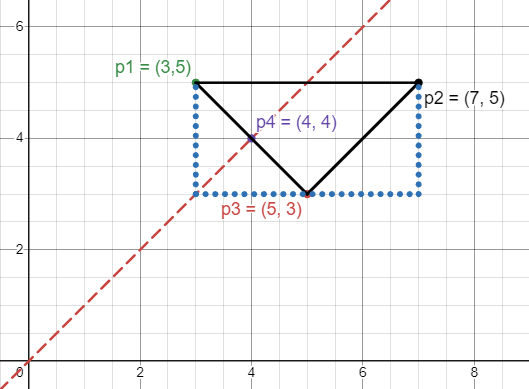
\includegraphics[width=0.5\linewidth]{q7_graph.png}
    \caption{Visual representation of the laser aim game, with relevant points, lines and edges}
    \label{fig:enter-label}
\end{figure}


\section*{Bonus Problem:}
For the solution to the bonus problem, I have first included some example graphs generated by my code, and then I have included a printout of the code used for this solution afterwards. 
The demonstrations used the following inputs:

\begin{figure}[H]
    \centering
    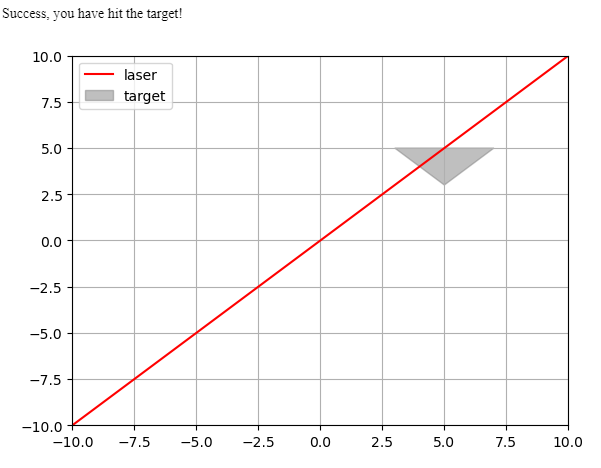
\includegraphics[width=0.42\linewidth]{original.png}
    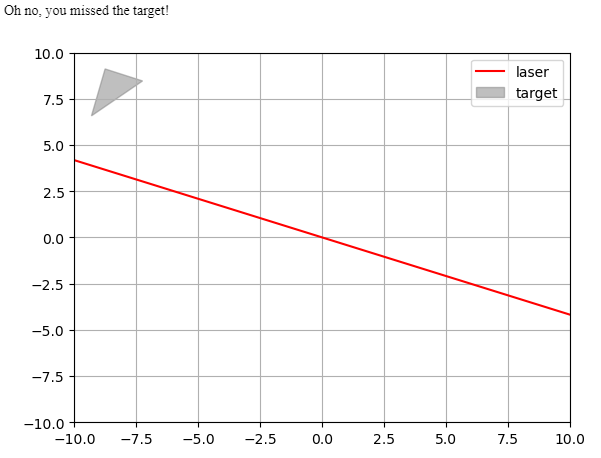
\includegraphics[width=0.42\linewidth]{miss.png}
    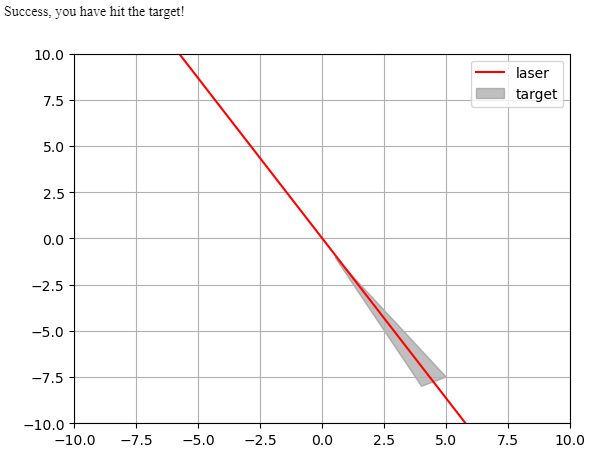
\includegraphics[width=0.42\linewidth]{bottom_right_demo.png}
    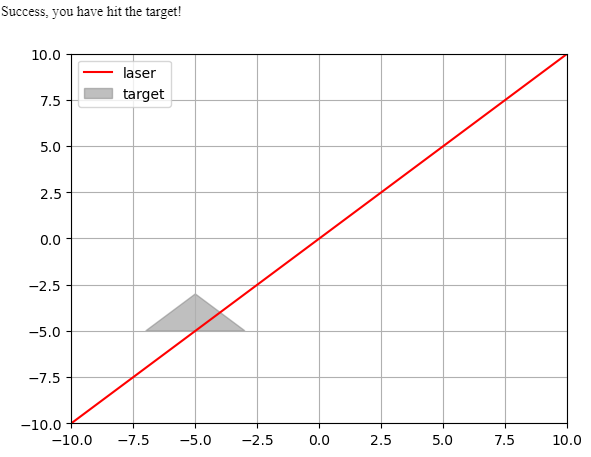
\includegraphics[width=0.42\linewidth]{succes_2.png}
    \caption{Python plots of the triangle and relevant laser, with a message informing the user if they hit or missed the target}
    \label{fig:enter-label}
\end{figure}

\subsection*{Code printout:}
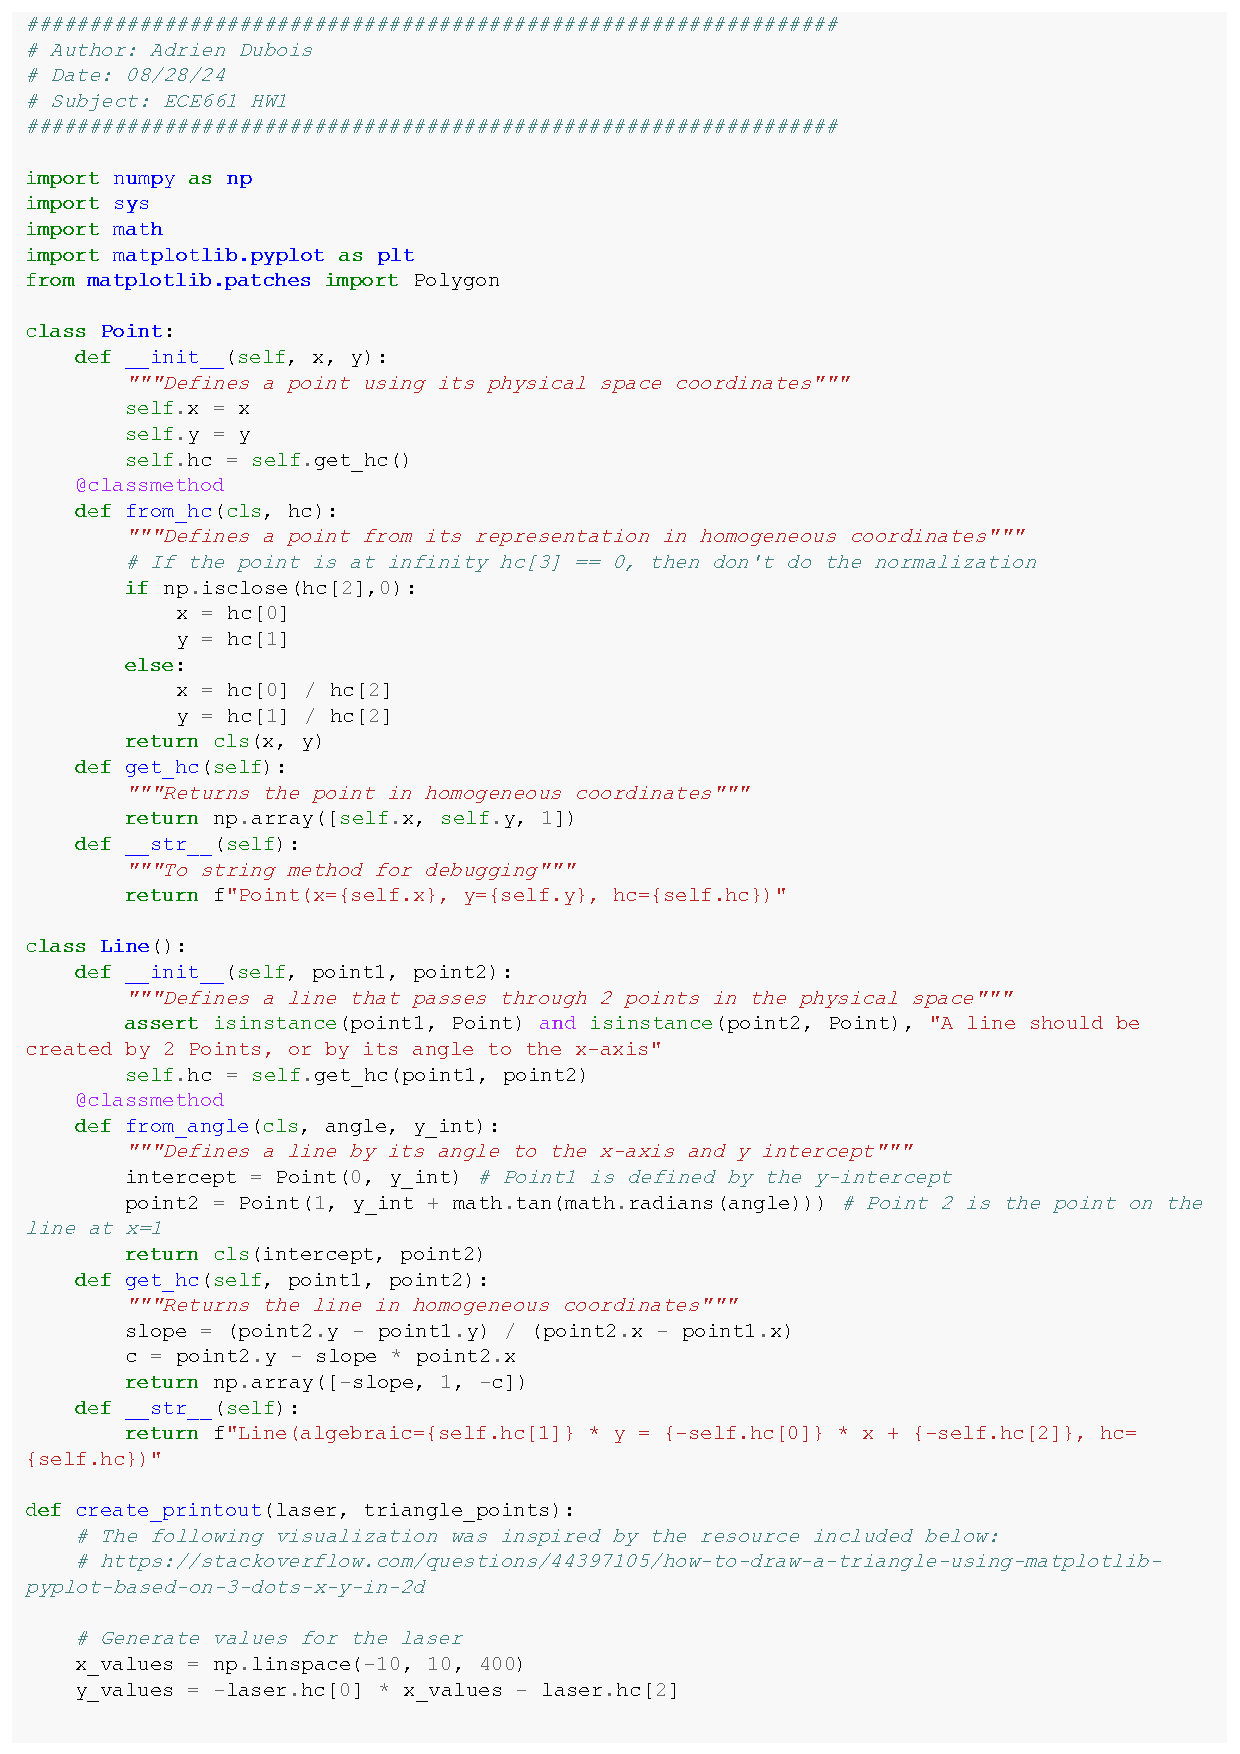
\includepdf[pages=-]{laser_aim_game.pdf}
\end{document}
